
\section{Univalence} \label{section:univalence}

In this section, we will introduce the Univalence Axiom, and show that it holds in the simplicial model.

The proof of this involves both simplicial and type-theoretic components; we keep these separate, as far as possible.  First of all (Section~\ref{subsec:type-theoretic-univalence}), we define univalence type-theoretically and state the Univalence Axiom; next, we define an analogous simplicial concept of univalence (Section~\ref{subsec:simplicial-univalence}); we then show that via the simplicial model, the two notions coincide (Section~\ref{subsec:univalence-equivalence}).  Finally, in Section~\ref{subsec:univalence-of-uu}, we prove our main theorem: that $\UU$ is univalent (using the simplicial sense), and hence that the Univalence Axiom holds in the simplicial model of type theory.  Lastly, in Section~\ref{subsec:pullback-reps}, we discuss an alternative formulation of simplicial univalence, and so obtain an up-to-homotopy uniqueness statement for the weak universal property of $\UU$.

Once again, we freely use the syntax of type theory as a notation; to avoid formal dependence on Conjecture~\ref{conj:initiality}, the reader should translate each individual syntactic expression used into the language of contextual categories.

\subsection{Type-theoretic univalence} \label{subsec:type-theoretic-univalence}

To state the univalence axiom, we first need to define a few basic notions in the type theory.

\begin{definition}[Joyal] \label{def:hiso} Let $f \colon A \to B$ be a function in some context $\Gamma$, i.e.\ $\Gamma\types f : [A,B]$ (where the function type $[A,B]$ is defined using $\synPi$, as described in Section~\ref{subsec:logical-rules}).
\begin{itemize}
\item A \emph{left homotopy inverse} for $f$ is a function $g \colon B \to A$, together with a homotopy $g \cdot f \homot 1_A$.  Formally, we define the type $\synLHInv(f)$ of left homotopy inverses to $f$:
\[ \Gamma \types \synLHInv(f) := \Sigma_{g \oftype [B,A]} \synPi_{x \oftype A} \synId_A(g(f(x)),x)\ \type \]

\item Analogously, we define the type $\synRHInv(f)$ of \emph{right homotopy inverses}:
\[ \Gamma \types \synRHInv(f) := \Sigma_{g \oftype [B,A]} \synPi_{y \oftype B} \synId_B(f(g(y)),y)\ \type \]

\item We say $f \colon A \to B$ is a \emph{homotopy isomorphism} (or more briefly, an h-isomorphism) if it is equipped with both a left and a right inverse:
\[ \Gamma \types \synisHIso(f) := \synLHInv(f) \times \synRHInv(f) \ \type \]

\item For any types $A$ and $B$, we thus have the type of h-isomorphisms from $A$ to $B$:
\[ \Gamma \types \synHIso(A,B) := \Sigma_{f \oftype [A,B]} \synisHIso(f) \]
\end{itemize}
\end{definition}

It may perhaps be surprising that we use homotopy isomorphisms rather than the more familiar homotopy equivalences, with a single two-sided homotopy inverse.  The reason is that while a map carries either structure if and only if it carries the other, the type, or object, of such structures on a map is different.  In particular, the analogue of Lemma~\ref{lemma:hiso-over-eq} for homotopy equivalences does not hold; for further discussion of these issues, see \cite[Ch.~4]{hott:book}.

\begin{example}
For any type $B$, the identity function on $B$ is canonically an h-isomorphism.
\end{example}

Suppose now that $A$ is any type, and $x \colon A \types B(x)\ \type$ a family of types over $A$.  By the identity elimination rule, we can derive
\[ x,y \oftype A,\ u \oftype \synId_A(x,y) \types w_{x,y,u} : \synHIso(B(x),B(y)). \]

This can equivalently be seen as a map
\[ x,y \oftype A \types w_{x,y} : [\synId_A(x,y), \synHIso(B(x),B(y))]. \]

\begin{definition} \label{def:type-theoretic-univalence}
We say the family $B(x)$ is \emph{univalent} if for each $x,y$, the map $w_{x,y}$ is itself a homotopy isomorphism:
\[ \types \synisUnivalent(x \oftype A . B(x)) := \synPi_{x,y \oftype A} \synisHIso(w_{x,y}). \]
\end{definition}

\begin{axiom} \label{axiom:univalence}
The \emph{Univalence Axiom}, for a given type-theoretic universe $U$, is the statement that the canonical family $\el$ of types over $U$ is univalent.
\end{axiom}

Informally, the Univalence Axiom says that just as elements of the universe correspond to types, so equalities in the universe correspond to equivalences between types.  In particular, since every statement or construction must respect propositional equality, the Univalence Axiom stipulates that the language can never distinguish between equivalent types.

\subsection{Simplicial univalence}  \label{subsec:simplicial-univalence}

To define a simplicial notion of univalence, we first need to construct the \emph{object of weak equivalences} between fibrations $p_1 \colon E_1 \to B$ and $p_2 \colon E_2 \to B$ over a common base.  In other words, we want an object representing the functor sending $(X,f) \in \sSets/B$ to the set $\extEq_X(f^*E_1,f^*E_2)$.  As we did for $\U$, we proceed in two steps, first exhibiting it as a subfunctor of a functor more easily seen (or already known) to be representable.

For the remainder of the section, fix fibrations $E_1$, $E_2$ as above over a base $B$. Since $\sSets$ is locally Cartesian closed, we can construct the exponential object between them:

\begin{definition} \label{def:internal-eq}
 Let $\intHom_B (E_1, E_2) \to B$ denote the internal hom from $E_1$ to $E_2$ in $\sSets/B$.

 Then for any $X$, a map $X \to \intHom_B (E_1,E_2)$ corresponds to a map $f \colon X \to B$, together with a map $u \colon f^*E_1 \to f^*E_2$ over $X$.

 Together with the Yoneda lemma, this implies the explicit description: an $n$-simplex of $\intHom_B (E_1,E_2)$ is a pair
 \[(b \colon \Delta[n] \to B, u \colon b^* E_1 \to b^* E_2) .\]
\end{definition}

\begin{lemma} \label{lemma:HOM_is_fib}
 $\intHom_B (E_1, E_2) \to B$ is a Kan fibration.
\end{lemma}

\begin{proof}
Follows immediately from Lemma~\ref{lemma:dep-prod-of-fibs}, since the exponential is a special case of dependent products.
\end{proof}

Within $\intHom_B (E_1, E_2)$, we now want to construct the subobject of weak equivalences.

\begin{lemma} \label{lemma:weqs_pull_back} %% VV Lemma 1.7
Let $f \colon E_1 \to E_2$ be a weak equivalence over $B$, and suppose $g \colon B' \to B$. Then the induced map between pullbacks $g^*E_1 \to g^*E_2$ is a weak equivalence.
\end{lemma}

\begin{proof}
The pullback functor $g^* \colon \sSets/B \to \sSets/B'$ preserves trivial fibrations; so by Ken Brown's Lemma \cite[Lemma~1.1.12]{hovey:book}, it preserves all weak equivalences between fibrant objects.
\end{proof}

Thus, weak equivalences from $E_1$ to $E_2$ form a subfunctor of the functor of maps from $E_1$ to $E_2$.  To show that this is representable, we need just to show:

\begin{lemma} \label{lemma:weq_fibers}  %% VV Lemma 1.8
 Let $f \colon E_1 \to E_2$ be a morphism over $B$.  If for each simplex $b \colon \Delta[n] \to B$ the induced map $f_b \colon b^*E_1 \to b^* E_2$ is a weak equivalence, then $f$ is a weak equivalence.
\end{lemma}

\begin{proof}
Without loss of generality, $B$ is connected; otherwise, apply the result over each connected component separately.  Take some vertex $b \colon \Delta[0] \to B$, and set $F_i := b^*E_i$.  Now for any vertex $e \colon \Delta[0] \to F_1$, and any $n \geq 1$, we have by the long exact sequence for a fibration:
 \[\mathclap{\xymatrix@C=0.5cm{
 \pi_{n+1} (B, b) \ar[r] \ar[d]_{1} & \pi_{n} (F_1, e) \ar[r] \ar[d]_{\pi_n (f_b)} & \pi_{n} (E_1, e) \ar[r] \ar[d]_{\pi_n(f)} & \pi_{n} (B, b) \ar[r] \ar[d]^{1} & \pi_{n-1} (F_1, e) \ar[d]^{\pi_{n-1} (f_b)} \\
 \pi_{n+1} (B, b) \ar[r] & \pi_{n} (F_2, f(e)) \ar[r] & \pi_{n} (E_2, f(e)) \ar[r] & \pi_{n} (B, b) \ar[r]  & \pi_{n-1} (F_2, f(e))  }}\]
Each $\pi_n(f_b)$ is an isomorphism, so by the Five Lemma, so is $\pi_n (f)$, for $n \geq 1$.  

The case $n = 0$ is the same in spirit, but requires a little more work since the Five Lemma is unavailable.  We have a square
 \[\xymatrix{
 \pi_0 (F_1) \ar@{->>}[r]^{\pi_0(i_1)} \ar[d]_{\pi_0 (f_b)} & \pi_0 (E_1) \ar[d]_{\pi_0 (f)} \\
 \pi_0 (F_2) \ar@{->>}[r]^{\pi_0(i_2)} & \pi_0 (E_2) }\]
with both horizontal arrows surjections, and $\pi_0(f_b)$ an isomorphism.  To show that $\pi_0(f)$ is an isomorphism, it therefore suffices to show that for each $x \in \pi_0(E_1)$, the restriction of $f_b$ to a map of fibers 
\[ \pi_0(i_1)^{-1}(x) \to \pi_0(i_2)^{-1}(\pi_0(f)(x)) \]
is again an isomorphism.  But this follows from the continuation of the long exact sequence to an exact sequence of pointed sets:
 \[\xymatrix{
 \pi_1(B,b) \ar[d]_{1} \ar[r] & \pi_0(F_1,e) \ar@{->>}[r]^{\pi_0(i_1)} \ar[d]_{\pi_0 (f_b)} & \pi_0(E_1,x) \ar[d]_{\pi_0 (f)} \\
 \pi_1(B,b) \ar[r] & \pi_0 (F_2,f(e))\ar@{->>}[r]^{\pi_0(i_2)} & \pi_0(E_2,f(e)) }\]
where $e$ is any point of $F_1$ such that $[e] = x$.

Thus $\pi_n(f)$ is an isomorphism for each $n \geq 0$ and basepoint $e \in E_1$; so $f$ is a weak equivalence.
\end{proof}

\begin{definition}
 Take $\intEq_B(E_1, E_2)$ to be the subobject of $\intHom_B (E_1, E_2)$ consisting of all $n$-simplices
 \[ (b \colon \Delta [n] \to B, w \colon b^*E_1 \to b^* E_2)\]
 such that $w$ is a weak equivalence.  (By Lemma~\ref{lemma:weqs_pull_back}, this indeed defines a simplicial subset.)
\end{definition}

From Lemma~\ref{lemma:weq_fibers}, we immediately have:

\begin{corollary}\label{cor:weqs_representable}
 Let $(f, u) \colon X \to \intHom_B (E_1, E_2)$.  Then $u$ is a weak equivalence if and only if $(f, u)$ factors through $\intEq_B (E_1, E_2)$.

 Thus, maps $X \to \intEq_B(E_1,E_2)$ correspond to pairs of maps
 \[(f \colon X \to B, w \colon f^*E_1 \to f^* E_2),\]
 where $w$ is a weak equivalence. \qed
\end{corollary}

While Lemma~\ref{lemma:weq_fibers} was stated just as required by representability, its proof actually gives a slightly stronger statement:

\begin{lemma} \label{lemma:connected_weq}  %% VV Lemma 1.10
 Let $f \colon E_1 \to E_2$ be a morphism over $B$.  If for some vertex $b \colon \Delta [0] \to B$ in each connected component the map of fibers $f_b \colon b^*E_1 \to b^* E_2$ is a weak equivalence, then $f$ is a weak equivalence. \qed
\end{lemma}

\begin{corollary} \label{cor:eq_is_fib}
 The map $\intEq_B(E_1,E_2) \to B$ is a fibration.
\end{corollary}

\begin{proof}
 Suppose we wish to fill a square:
 \[\xymatrix{ \Lambda^k[n] \ar[r] \ar@{^{(}->}[d]^i & \intEq_B(E_1,E_2) \ar[d] \\ % } to match brackets
  \Delta[n] \ar@{.>}[ur] \ar[r]^b & B \\
 }\]
 By the universal property of $\intEq_B(E_1,E_2)$ this corresponds to showing that we can extend a weak equivalence $w \colon i^*b^*E_1 \to i^*b^*E_2$ over $\Lambda^k[n]$ to a weak equivalence $\overline{w} \colon b^*E_1 \to b^*E_2$ over $\Delta[n]$.

 By Lemma~\ref{lemma:HOM_is_fib}, we can certainly find some map $\overline{w}$ extending $w$.  But then since $\Delta[n]$ is connected, Lemma~\ref{lemma:connected_weq} implies that $\overline{w}$ is a weak equivalence.
\end{proof}

While on the subject, we collect a proposition which is not required for the definition of univalence, but which will be useful later:
\begin{proposition} \label{prop:eq-respects-weq}
Suppose that $E_1,E_1',E_2,E_2'$ are fibrations over a common base $B$, and $w_1 \colon E'_1 \to E_1$, $w_2 \colon E_2 \to E'_2$ are weak equivalences over $B$.  Then the induced map $\intEq_B(w_1,w_2) \colon \intEq_B (E_1,E_2) \to \intEq_B (E'_1,E'_2)$ is a weak equivalence.

\[ 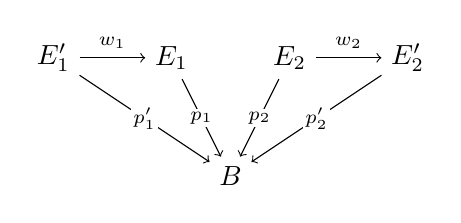
\begin{tikzpicture}[hole/.style={fill=white,inner sep=1pt},x=1.5cm,y=1.5cm]
\node (E1') at (0,1) {$E'_1$};
\node (E1) at (1,1) {$E_1$};
\node (E2) at (2,1) {$E_2$};
\node (E2') at (3,1) {$E'_2$};
\node (B) at (1.5,0) {$B$};
\draw[->,font=\scriptsize] (E1') to node[hole] {$p'_1$} (B);
\draw[->,font=\scriptsize] (E1) to node[hole] {$p_1$} (B);
\draw[->,font=\scriptsize] (E2) to node[hole] {$p_2$} (B);
\draw[->,font=\scriptsize] (E2') to node[hole] {$p'_2$} (B);
\draw[->,font=\scriptsize,auto] (E1') to node {$w_1$} (E1);
\draw[->,font=\scriptsize,auto] (E2) to node {$w_2$} (E2');
\end{tikzpicture} \]
\end{proposition}

\begin{proof}
As weak equivalences between fibrations, $w_1$ and $w_2$ are fibered homotopy equivalences over $B$.  Choosing fibered homotopy inverses $v_1$, $v_2$ for $w_1$ and $w_2$ respectively gives a homotopy inverse $\intHom_B(v_1,v_2)$ for $\intHom_B(w_1,w_2) \colon \intHom_B (E_1,E_2) \to \intHom_B (E'_1,E'_2)$.  But by Lemma~\ref{lemma:connected_weq}, the image of a homotopy in $\intHom$ whose endpoints lie in $\intEq$ must lie entirely in $\intEq$; so the restriction $\intEq_B(v_1,v_2)$  gives a homotopy inverse for $\intEq_B(w_1,w_2)$, as desired.
\end{proof}

We are now ready to define univalence.

Let $p \colon E \to B$ be a fibration.  We then have two fibrations over $B \times B$, given by pulling back $E$ along the projections.  Call the object of weak equivalences between these $\intEq(E) := \intEq_{B \times B}(\pi_1^*E,\pi_2^*E)$.  Concretely, simplices of $\intEq(E)$ are triples
\[ (b_1,b_2 \in B_n,\, w \colon b_1^*E \to b_2^*E ). \]

By Corollary~\ref{cor:weqs_representable}, a map $f \colon X \to \intEq(E)$ corresponds to a pair of maps $f_1, f_2 \colon X \to B$ together with a weak equivalence $f_1^*E \to f_2^*E$ over $X$.  In particular, there is a “diagonal” map $\delta_E \colon B \to \intEq(E)$ corresponding to the triple $(1_B,1_B,1_E)$, sending a simplex $b \in B_n$ to the triple $(b,b,1_{E_b})$.

There are also source and target maps $s,t \colon \intEq(E) \to B$, given by the composites $\intEq(E) \to B \times B \to^{\pi_i} B$, sending $(b_1,b_2,w)$ to $b_1$ and $b_2$ respectively.  These are both retractions of $\delta$; and by Corollary~\ref{cor:eq_is_fib}, if $B$ is fibrant then they are moreover fibrations.

\begin{definition} \label{def:simplicial-univalence}
 A fibration $p \colon E \to B$ is \emph{univalent} if the diagonal map $\delta_E \colon B \to \intEq (E)$ is a weak equivalence.
\end{definition}

Since $\delta_E$ is always a monomorphism (thanks to its retractions), this is equivalent to saying that $B \to \intEq(E) \to B \times B$ is a (trivial cofibration, fibration) factorisation of the diagonal $\Delta_B \colon B \to B \times B$, i.e.\ that $\intEq(E)$ is a \emph{path object} for $B$.

We conclude this section with a few examples, and non-examples, of univalent fibrations.

\begin{examples} \leavevmode
\begin{enumerate}
  \item The canonical map $X \to 1$ is univalent if and only if the space of homotopy auto-equivalences of $X$ is contractible.
% Remove unless we can find a good reference: In particular, for a group $G$, the map $\B G \to 1$ is univalent just if the center and group of outer automorphisms of $G$ are trivial, as for instance in the case $G = S_n$.
  \item The identity map $X \to X$ is univalent if and only if $X$ is either empty or contractible.  In particular, the identity map $1 + 1 \to 1 + 1$ is \emph{not} univalent: it has two fibers which are equivalent, over points that are not connected by any path.
  \item Any fibration weakly equivalent to a univalent fibration is itself univalent (essentially, by Proposition~\ref{prop:eq-respects-weq}).
\end{enumerate}
\end{examples}

\subsection{Equivalence of type-theoretic and simplicial univalence} \label{subsec:univalence-equivalence}

Having defined the type-theoretic and simplicial notions of univalence, we now wish to show that they coincide.  As ever, we make essential use of representability; in particular, we work with the interpretations of type-theoretic notions entirely via their universal properties.  With this in view, we need to define what are represented by the interpretations of $\synLHInv$, $\synisHIso$, etc.

\begin{definition}
Let $p_1 \colon E_1 \to B$, $p_2 \colon E_2 \to B$ be fibrations over a common base (as in Definition~\ref{def:internal-eq}).

Define $\extHomLHInv_B(E_1,E_2)$ to be the set of \emph{maps with a left homotopy inverse} from $E_1$ to $E_2$, i.e.\ triples $(f,g,H)$, where $f \colon E_1 \to E_2$ and $g \colon E_2 \to E_1$ are maps over $B$, and $H$ is a fibred homotopy from $g \cdot f$ to $1_{E_1}$, defined using the fibred path space $\paths_B(E_1)$ (as used for the $\IdStrux$-structure in the proof of Theorem~\ref{thm:the-model-in-ssets}).

Similarly, define $\extHomRHInv_B(E_1,E_2)$ to consist of triples $(f,g,H)$, where $f, g$ are as before, and $H$ is now a fibred homotopy from $f \cdot g$ to $1_{E_2}$, defined using $\paths_B(E_2)$.

Finally, these both come with evident projections to $\Hom_B(E_1,E_2)$; define $\extHIso_B(E_1,E_2)$ as the pullback $\extHomLHInv_B(E_1,E_2) \times_{\Hom_B(E_1,E_2)} \extHomRHInv_B(E_1,E_2).$
\end{definition}

\begin{lemma} \label{lemma:interpretation_correct}
Let $B,E_1,E_2$ be as above; additionally, suppose they are given by names $\name{B} \colon 1 \to \UU$, $\name{E_i} \colon B \to \UU$.  Then for any $f \colon X \to B$, there are horizontal isomorphisms as in the diagram below, making the diagram commute, and natural in $(X,f)$.

% editing note: width may be easily adjusted by changing defn of x at start.
\[\mathclap{\begin{tikzpicture}[x={(7cm,0cm)},y={(1.8cm,-1.8cm-1em)},z={(1.8cm,1.8cm-1em)}]
  % objects from the type theory:
  \node (tMap) at (0,0,0) {$\Hom_B(X,\interp{ [E_1,E_2] } )$};
  \node (tLInv) at (0,-1,0) {$\Hom_B(X,\interp{ \synHomLHInv(E_1,E_2) } )$};
  \node (tRInv) at (0,0,1) {$\Hom_B(X,\interp{ \synHomRHInv(E_1,E_2) }) $};
  \node (tHEq) at (0,-1,1) {$\Hom_B(X,\interp{ \synHIso(E_1,E_2) }) $};
  \draw[->] (tLInv) to (tMap);
  \draw[->] (tRInv) to (tMap);
  \draw[->] (tHEq) to (tLInv);
  \draw[->] (tHEq) to (tRInv);
  \draw (0,-0.92,0.8) -- (0,-0.84,0.8) -- (0,-0.84,0.9); % pullback sign
 % objects defined directly in sets:
  \node (sMap) at (1,0,0) {$\Hom_X(f^*E_1,f^*E_2)$};
  \node (sLInv) at (1,-1,0) {$\extHomLHInv_X(f^*E_1,f^*E_2)$};
  \node (sRInv) at (1,0,1) {$\extHomRHInv_X(f^*E_1,f^*E_2)$};
  \node (sHEq) at (1,-1,1) {$\extHIso_X(f^*E_1,f^*E_2)$};
  \draw[->] (sLInv) to (sMap);
  \draw[->] (sRInv) to (sMap);
  \draw[->] (sHEq) to (sLInv);
  \draw[->] (sHEq) to (sRInv);
  \draw (1,-0.92,0.8) -- (1,-0.84,0.8) -- (1,-0.84,0.9); % pullback sign
% connecting arrows:
  \draw[->,dotted] (tMap) to node {$\iso$} (sMap);
  \draw[->,dotted] (tLInv) to node {$\iso$}  (sLInv);
  \draw[->,dotted] (tRInv) to node {$\iso$}  (sRInv);
  \draw[->,dotted] (tHEq) to node {$\iso$}  (sHEq);
\end{tikzpicture}}\]

(Here $\interp{-}$ denotes the interpretation of type theory, as described following Corollary~\ref{cor:simplicial-model}; and $[-,-]$ is the ordinary function type, taken as a special case of $\Pi$-types.)
\end{lemma}

\begin{proof} This is essentially a routine verification; we prove just the first case, that of $\interp{ [ {E_1}, {E_2}] }$.  For this, we need to give a natural isomorphism $\Hom_B( X, \interp{ [ {E_1}, {E_2}] } ) \iso \Hom_X(f^*E_1, f^*E_2)$; in other words, to show that $\interp{ [ {E_1}, {E_2}] }$ is the exponential between $E_1$ and $E_2$ in $\sSets/B$.

Recall that by definition, $\interp{ [ {E_1}, {E_2}] }$ is constructed as the pullback of $\UUt$ along the map $\PiStrux \cdot \name{(E_1,E_2)} \colon B \to \UU$:
\[\xymatrix{ 
\interp{ [{E_1}, {E_2} ] } \ar[d] \ar[r] \pb & \toposPi_{A_\gen \shortto B_\gen} B_\gen \ar[d] \ar[r] \pb & \UUt \ar[d] \\
B \ar[r]^-{\name{(E_1,E_2)}} & \UU^{\synPi\text{-}\form} \ar[r]^-\PiStrux & \UU
}\]

$\interp{ [ E_1, E_2] }$ is thus a pullback of the dependent product of the universal pair of fibrations over $\UU^{\synPi\text{-}\form}$, and so by the Beck-Chevalley condition is a dependent product for the pullbacks of these fibrations along $\name{(E_1,E_2)}$.  But these pullbacks are isomorphic to $E_1$, $E_1 \times_B E_2$, by the two pullbacks lemma and the construction of $A_\gen$, $B_\gen$ as pullbacks of $\UUt \to \UU$.

\[\mathclap{\begin{tikzpicture}[x={(6cm,0cm)},y={(-0.8cm,1.5cm+0.7em)},z={(0.6cm,1.5cm-0.7em)}]
  % objects from the type theory:
  \node (B) at (0,0,0) {$B$};
  \node (PiE1E2) at (0,1,0) {$\Pi_{E_1}(E_1^* E_2) $};
  \node (E1) at (0,0,1) {$E_1$};
  \node (E1E2) at (0,0,2) {$E_1^* E_2$};
  \draw[->] (PiE1E2) to (B);
  \draw[->] (E1) to (tMap);
  \draw[->] (E1E2) to (E1);
% objects defined directly in sets:
  \node (UPiForm) at (1,0,0) {$\UU^{\synPi\text{-}\form}$};
  \node (PiGen) at (1,1,0) {$\Pi_{A_\gen} B_\gen$};
  \node (AGen) at (1,0,1) {$A_\gen$};
  \node (BGen) at (1,0,2) {$B_\gen$};
  \draw[->] (PiGen) to (UPiForm);
  \draw[->] (AGen) to (UPiForm);
  \draw[->] (BGen) to (AGen);
% connecting arrows:
  \draw[->] (B) to (UPiForm);
  \draw[->] (PiE1E2) to (PiGen);
  \draw (0.04,0.74,0) -- (0.08,0.74,0) -- (0.08,0.87,0);
  \draw[->] (E1) to (AGen);
  \draw (0.04,0,0.66) -- (0.08,0,0.66) -- (0.08,0,0.83);
  \draw[->] (E1E2) to (BGen);
  \draw (0.04,0,1.66) -- (0.08,0,1.66) -- (0.08,0,1.83);
\end{tikzpicture} } \]

So $\interp{ [ {E_1}, {E_2}] }$ is the dependent product of $E_1 \times_B E_2 \to E_1$ along $E_1 \to B$; but this is exactly the usual construction of exponentials in slices from dependent products \cite[A1.5.2]{johnstone:elephant-i}.
\end{proof}

We also note, from the proof of the preceding lemma:
\begin{corollary}
There is a natural isomorphism over $B$:
\[\interp{ [E_1,E_2] } \iso \intHom_B(E_1,E_2). \extraqedhere \]
\end{corollary}

Following this, we define $\intHIso_B(E_1,E_2) := \interp{ \synHIso_B(E_1,E_2) }$, and $\intHomLHInv$, $\intHomRHInv$ similarly.

\begin{lemma} \label{lemma:hiso-over-eq}
The map $ \intHIso_B(E_1,E_2) \to \intHom_B(E_1,E_2)$ factors through $\intEq_B(E_1,E_2)$; and the resulting map $ \intHIso_B(E_1,E_2) \to \intEq_B(E_1,E_2)$ is a trivial fibration.
\end{lemma}

\begin{proof}
The given map  $ \intHIso_B(E_1,E_2) \to [E_1,E_2] \iso \intHom_B(E_1,E_2)$ corresponds, under the isomorphisms of Lemma~\ref{lemma:interpretation_correct}, to the maps on hom-sets
\begin{equation}
\begin{split}
\Hom_B (X, \intHIso_B (E_1, E_2)) & \iso \extHIso_X (f^*E_1, f^*E_2) \\
& \to \Hom_X (f^*E_1, f^*E_2) \\
& \iso \Hom_B (X, \intHom_B(E_1, E_2)) 
\end{split}
\end{equation}
where the middle map just forgets the chosen homotopy inverses of an h-isomorphism.  But since any map admitting both homotopy inverses is a weak equivalence, the natural map
\[\extHIso_X (f^*E_1, f^*E_2) \to \Hom_X (f^*E_1, f^*E_2)\]
factors through $\extEq_X (f^*E_1, f^*E_2)$; so by Yoneda, $\intHIso_B(E_1,E_2) \to \intHom_B(E_1,E_2)$ factors through $\intEq_B(E_1,E_2)$.
 
Thus, we obtain the desired map $\intHIso_B(E_1, E_2) \to \intEq_B (E_1, E_2)$, corresponding to the forgetful function $\extHIso_X (f^*E_1, f^*E_2) \to \extEq_X (f^*E_1, f^*E_2)$.

Combining this with the left-hand pullback square in Lemma~\ref{lemma:interpretation_correct}, we can consider $\intHIso_B(E_1,E_2)$ as the pullback:
\[\mathclap{\begin{tikzpicture}[x={(-2.4cm,1.6cm)},y={(2.8cm,1.2cm)},z={(0,2.4cm)}]
 \node (Hom) at (0,0,0) {$\intHom_B(E_1,E_2)$};
  \node (HomLInv) at (1,0,0) {$\intHomLHInv_B(E_1,E_2)$};
  \draw[->] (HomLInv) to (Hom);
  \node (HomRInv) at (0,1,0) {$\intHomRHInv_B(E_1,E_2)$};
  \draw[->] (HomRInv) to (Hom);
  \node (Eq) at (0,0,1) {$\intEq_B(E_1,E_2)$};
  \draw[->] (Eq) to (Hom);
  \node (EqLInv) at (1,0,1) {$\intEqLHInv_B(E_1,E_2)$};
  \draw[->] (EqLInv) to (HomLInv);
  \draw[->] (EqLInv) to (Eq);
  \draw (0.9,0,0.8) -- (0.8,0,0.8) -- (0.8,0,0.9); 
  \node (EqRInv) at (0,1,1) {$\intEqRHInv_B(E_1,E_2)$};
  \draw[->] (EqRInv) to (Eq);
  \draw[->] (EqRInv) to (HomRInv);
  \draw (0,0.9,0.8) -- (0,0.8,0.8) -- (0,0.8,0.9); 
  \node (HIso) at (1,1,1) {$\intHIso_B(E_1,E_2)$};
  \draw[->] (HIso) to (EqLInv);
  \draw[->] (HIso) to (EqRInv);
  \draw (0.9,0.8,1) -- (0.8,0.8,1) -- (0.8,0.9,1); 
\end{tikzpicture} } \]
where $\intEqLHInv$, $\intEqRHInv$ are defined by the pullbacks above, and represent weak equivalences equipped with a left (resp.\ right) homotopy inverse.  To show that $\intHIso_B(E_1, E_2) \to$ $\intEq_B (E_1, E_2)$ is a trivial fibration, it thus suffices to show that the maps
 \begin{eqnarray*}
   \intEqLHInv_B (E_1, E_2) & \to & \intEq_B (E_1, E_2) \\
   \intEqRHInv_B (E_1, E_2) & \to & \intEq_B (E_1, E_2)
\end{eqnarray*}
are each trivial fibrations.  We show this in the following two lemmas. 

\begin{lemma} \label{lemma:lhinv-over-eq}
For $B$, $E_1$, $E_2$ as above, the map 
\[\intEqLHInv_B (E_1, E_2) \to \intEq_B (E_1, E_2)\]
is a trivial fibration.  Equivalently, left homotopy inverses to equivalences between fibrant objects extend along cofibrations.
\end{lemma}

\begin{proof}
For $\intEqLHInv_B (E_1, E_2) \to \intEq_B (E_1, E_2)$, we need to find a filler for any diagram of the form
 \[\xymatrix{Y \ar[rr] \ar@{^{(}->}[d]_i & & \intEqLHInv_B (E_1, E_2) \ar[d] \\
 X \ar[rr] \ar@{..>}[rru] & & \intEq_B(E_1, E_2)  }\]
where  $i \colon Y \into X$ is a cofibration.

Writing $f$ for the induced map $X \to B$ and $F_i$ for $f^*E_i$, this square corresponds (by the universal properties of $\intEq$ and $\intEqLHInv$) to a weak equivalence $\bar{w} \colon F_1 \to F_2$, and a fibered left homtopy inverse to $w := i^* \bar{w}$; that is, $l \colon i^* F_2 \to i^* F_1$, and a homotopy $H \colon l \cdot w \homot 1_{i^*F_1}$, all fibered over $Y$:
\[\begin{tikzpicture}[hole/.style={fill=white,inner sep=1pt},x={(1.5cm,0cm)},y={(0cm,1.8cm)},z={(1.8cm,-0.7cm)}]
  % part over Y:
  \node (Y) at (0,0,0) {$Y$};
  \node (iF1) at (0,1,-0.5) {$i^*F_1$};
  \node (iF2) at (0,1,0.5) {$i^*F_2$};
  \draw[->] (iF1) to (Y);
  \draw[->] (iF2) to (Y);
  \draw[->,bend left=12,font=\scriptsize] (iF1) to node[hole] {$w$} (iF2);
  \draw[->,bend left=32,font=\scriptsize] (iF2) to node[hole] {$l$} (iF1);
%  \draw[->,bend left=10,font=\scriptsize,double equal sign distance,-implies,shorten >=1pt,shorten <=3pt]
%      (iF2) to node[hole] {$H$} (iF1); 
  % part over X:
  \node (X) at (2,0,0) {$X$};
  \node (F1) at (2,1,-0.5) {$F_1$};
  \node (F2) at (2,1,0.5) {$F_2$};
  \draw[->] (F1) to (X);
  \draw[->] (F2) to (X);
  \draw[->,bend left=12,auto] (F1) to node {$\scriptstyle \overline{w}$} (F2);
  % connecting arrows:
  \draw[c'->] (Y) to (X);
  \draw[c'->] (iF2) to (F2);
  \draw (0.2,0.7,0.35) -- (0.4,0.7,0.35) -- (0.4,0.85,0.425); % pullback sign
  \draw[c'->] (iF1) to (F1);
%  \draw (0.2,0.8,-0.4) -- (0.4,0.8,-0.4) -- (0.4,0.9,-0.45); % pullback sign
\end{tikzpicture}\]
A filler then corresponds to a fibered left homotopy inverse $(\bar{l},\bar{H})$ to $\bar{w}$, extending $(l,H)$.

These data and desiderata may be summed up in a single commuting diagram:
\[\begin{tikzpicture}[x={(1.8cm,0)},y={(0,-1.2cm)}]
% top left:
\node (F1tl) at (2,0) {$F_1$};
\node (iF1) at (1,0) {$i^* F_1$};
\node (iF1xI) at (1,1) {$i^* F_1 \times \Delta[1]$};
\node (iF1') at (0,1) {$i^* F_1$};
\node (iF2) at (0,2) {$i^*F_2$};
\draw[right hook->,auto] (iF1) to (F1tl);
\draw[->,auto] (iF1) to node {$\scriptstyle \iota_1$} (iF1xI);
\draw[->,auto] (iF1') to node {$\scriptstyle \iota_0$} (iF1xI);
\draw[->,auto] (iF1') to node {$\scriptstyle w$} (iF2);
% top right:
\node (iF1tr) at (4.5,1) {$i^*F_1$};
\node (F1tr) at (6,1) {$F_1$};
\draw[->] (iF1tr) to (F1tr);
% bottom left:
\node (F1xI) at (1.5,5) {$F_1 \times \Delta[1]$};
\node (F1bl) at (0.5,5) {$F_1$};
\node (F2) at (0.5,4) {$F_2$};
\draw[->,auto] (F1bl) to node {$\scriptstyle \bar{w}$} (F2);
\draw[->,auto] (F1bl) to node {$\scriptstyle \iota_0$} (F1xI);
% bottom right;
\node (F1br) at (4.5,5) {$F_1$};
\node (X) at (6,5) {$X$};
\draw[->] (F1br) to (X);
% top row:
\draw[->,auto] (F1tl) to node {$\scriptstyle 1$} (F1tr);
\draw[->,auto] (iF1xI) to node {$\scriptstyle H$} (iF1tr);
\draw[->,auto] (iF2) to node {$\scriptstyle l$} (iF1tr);
% left column:
\draw[right hook->] (iF2) to (F2);
\draw[right hook->] (iF1xI) to (F1xI);
\draw[->,auto] (F1tl) to node {$\scriptstyle \iota_1$} (F1xI);
% bottom row:
\draw[->,auto] (F1xI) to node {$\scriptstyle \pi_1$} (F1br);
\draw[->] (F2) to (X);
% right column:
\draw[->] (F1tr) to (X);
% diagonal:
\draw[->,dotted,auto] (F2) to node {$\scriptstyle \bar{l}$} (F1tr);
\draw[->,dotted,auto] (F1xI) to node {$\scriptstyle  H$} (F1tr);
\end{tikzpicture}\]

Replacing the sub-diagrams on the left by their colimits, we see that we seek precisely a diagonal filler for an associated square:
\[\xymatrix{
 i^*F_2 +_{i^*F_1} (i^*F_1 \times \Delta[1]) +_{i^*F_1} F_1 \ar[rr] \ar[d] & & F_1 \ar[d] \\
 F_2 +_{F_1} (F_1 \times \Delta[1]) \ar@{..>}[urr] \ar[rr] & & X
}\]
So since $F_1 \to X$ is a fibration, we just need to show that the left-hand map of pushouts, induced by
\[\begin{tikzpicture}[x={(1.8cm,0)},y={(0,-1.2cm)}]
% top left:
\node (F1tl) at (2,0) {$F_1$};
\node (iF1) at (1,0) {$i^* F_1$};
\node (iF1xI) at (1,1) {$i^* F_1 \times \Delta[1]$};
\node (iF1') at (0,1) {$i^* F_1$};
\node (iF2) at (0,2) {$i^*F_2$};
\draw[->,auto] (iF1) to (F1tl); % should be “into”
\draw[->,auto] (iF1) to node {$\scriptstyle \iota_1$} (iF1xI);
\draw[->,auto] (iF1') to node {$\scriptstyle \iota_0$} (iF1xI);
\draw[->,auto] (iF1') to node {$\scriptstyle w$} (iF2);
% bottom left:
\node (F1xI) at (2.5,2.5) {$F_1 \times \Delta[1]$};
\node (F1bl) at (1.5,2.5) {$F_1$};
\node (F2) at (1.5,3.5) {$F_2$};
\draw[->,auto] (F1bl) to node {$\scriptstyle \bar{w}$} (F2);
\draw[->,auto] (F1bl) to node {$\scriptstyle \iota_0$} (F1xI);
% left column:
\draw[right hook->] (iF2) to (F2);
\draw[right hook->] (iF1') to (F1bl);
\draw[right hook->] (iF1xI) to (F1xI);
\draw[->,auto] (F1tl) to node {$\scriptstyle \iota_1$} (F1xI);
\end{tikzpicture} \]
is a trivial cofibration.  For convenience, call this map $t$.
 
To see that $t$ is a weak equivalence, consider it in the square
\[\xymatrix{
 (i^*F_1 \times \Delta[1]) +_{i^*F_1} F_1 \ar[r] \ar[d] & F_1 \times \Delta[1] \ar[d] \\
 i^*F_2 +_{i^*F_1} ((i^*F_1 \times \Delta[1] ) +_{i^*F_1} F_1) \ar[r]^-t & F_2 +_{F_1} (F_1 \times \Delta[1]).
}\]
The top map is a trivial cofibration by the pushout-product property; the vertical maps are pushouts of $w$ and $\bar{w}$ along cofibrations, so are also weak equivalences; and so by 2-out-of-3, $t$ is a weak equivalence.

On that other hand, to see that $t$ is a cofibration, consider it as induced by maps $t_0$, $t_1$ as in:
\[\xymatrix{
 i^*F_1 \ar[r] \ar[d] & F_1 \ar[d]^{t_1} \\
 i^*F_2 +_{i^*F_1} (i^*F_1 \times \Delta[1] ) \ar[r]^-{t_0} & F_2 +_{F_1} (F_1 \times \Delta[1]).
}\]
Here $t_0$ is isomorphic to the inclusion 
\[ i^*(F_2 +_{F_1} (F_1 \times \Delta[1])) \into F_2 +_{F_1} (F_1 \times \Delta[1])\]
(since pulling back preserves products and pushouts), so is mono.  Next, $i_0$ and $i_1$ have disjoint images, so $t_1$ is also mono.  Finally, the intersection of the images of $t_0$ and $t_1$ is exactly the image of $i^*F_1$; so $t$, as the induced map from $(i^*F_2 +_{i^*F_1} (i^*F_1 \times \Delta[1] )) +_{i^*F_1} F_1$, is mono as desired.

Thus $t$ is a trivial cofibration, completing the proof of the lemma.
\end{proof}
 
\begin{lemma} \label{lemma:rhinv-over-eq}
For $B$, $E_1$, $E_2$ as above, the map 
\[ \intEqRHInv_B (E_1, E_2) \to \intEq_B (E_1, E_2)\]
is a trivial fibration.  Equivalently, right homotopy inverses to equivalences between fibrant objects extend along cofibrations.
\end{lemma}
 
\begin{proof}
We must provide lifts against any cofibration $i \colon Y \into X$:
 \[\xymatrix{Y \ar[rr] \ar@{^{(}->}[d]_i & & \intEqRHInv_B (E_1, E_2) \ar[d] \\
 X \ar[rr] \ar@{..>}[rru] & & \intEq_B(E_1, E_2) }\]

Analogously to the previous lemma, and again writing $f \colon X \to B$, $F_i := f^* E_1$, the square corresponds to a weak equivalence $\bar{w} \colon F_1 \to F_2$ over $X$ together with a fibered right homotopy inverse to $w := i^* \bar{w}$, i.e.\ $r \colon i^*F_2 \to i^*F_1$ and a homotopy $H \colon w \cdot r \homot 1_{i^*F_2}$ over $Y$;
\[\begin{tikzpicture}[hole/.style={fill=white,inner sep=1pt},x={(1.5cm,0cm)},y={(0cm,1.8cm)},z={(1.8cm,-0.7cm)}]
  % part over Y:
  \node (Y) at (0,0,0) {$Y$};
  \node (iF1) at (0,1,-0.5) {$i^*F_1$};
  \node (iF2) at (0,1,0.5) {$i^*F_2$};
  \draw[->] (iF1) to (Y);
  \draw[->] (iF2) to (Y);
  \draw[->,bend left=12,font=\scriptsize] (iF1) to node[hole] {$w$} (iF2);
  \draw[->,bend left=32,font=\scriptsize] (iF2) to node[hole] {$r$} (iF1);
%  \draw[->,bend right=10,font=\scriptsize,double equal sign distance,-implies,shorten >=1pt,shorten <=3pt]
%      (iF1) to node[hole] {$H$} (iF2); 
  % part over X:
  \node (X) at (2,0,0) {$X$};
  \node (F1) at (2,1,-0.5) {$F_1$};
  \node (F2) at (2,1,0.5) {$F_2$};
  \draw[->] (F1) to (X);
  \draw[->] (F2) to (X);
  \draw[->,bend left=12,auto] (F1) to node {$\scriptstyle \overline{w}$} (F2);
  % connecting arrows:
  \draw[c'->] (Y) to (X);
  \draw[c'->] (iF2) to (F2);
  \draw (0.2,0.7,0.35) -- (0.4,0.7,0.35) -- (0.4,0.85,0.425); % pullback sign
  \draw[c'->] (iF1) to (F1);
%  \draw (0.2,0.8,-0.4) -- (0.4,0.8,-0.4) -- (0.4,0.9,-0.45); % pullback sign
\end{tikzpicture}\]
and a filler corresponds to a fibered right homotopy inverse $(\bar{r},\bar{H})$ for $\bar{w}$, extending $(r,H)$.

Again, putting these conditions together, we see that they correspond to filling another square:
\[\xymatrix{
  i^*F_2 \ar[r]^-{(r,H)} \ar[d] & i^*F_1 \times_{i^*F_2} \paths_Y (i^*F_2) \ar[r] & F_1 \times_{F_2} \paths_X F_2  \ar[d]^{\ev_1 \cdot \pi_1} \\
  F_2 \ar[rr]^1 \ar@{..>}[urr]|{(\bar{r},\bar{H})} & & F_2
}\]
where the pullbacks are just the fibered mapping path spaces.
\[\xymatrix{
  i^*F_1 \times_{i^*F_2} \paths_Y (i^*F_2) \ar[d] \ar[r] \pb & \paths_Y(i^*F_2) \ar[d]^{\ev_0} \\
  i^*F_1 \ar[r]^w  & i^*F_2
} \qquad
\xymatrix{
  F_1 \times_{F_2} \paths_X F_2 \ar[d] \ar[r] \pb & \paths_Y F_2 \ar[d]^{\ev_0} \\
  F_1 \ar[r]^{\bar{w}}  & F_2
}\]

Now $i^*F_2 \into F_2$ is certainly a cofibration; so to provide the filler, it suffices to show that the right-hand map is a trivial fibration.  As the target map from a mapping path space, it is certainly a fibration.  To see that it is a weak equivalence, consider the triangle 
\[ \xymatrix@C=3cm{
  F_1 \ar[r]^-{x\; \mapsto\; (x,c_{\bar{w}x})} \ar[dr]_{\bar{w}} & F_1 \times_{F_2} \paths_X F_2 \ar[d]^{\ev_0} \\
  & F_2 
}\]
The top map is the inclusion of a deformation retraction, so is a weak equivalence; so by 2-out-of-3, the source map $\ev_0$ is a  weak equivalence.  But $\ev_1$ is homotopic to $\ev_0$, so is also a weak equivalence, as required.
\end{proof}

Putting these two lemmas together concludes the proof of Lemma~\ref{lemma:hiso-over-eq}: $\intHIso$ is trivially fibrant over $\intEq$.
\end{proof}

\begin{theorem} \label{thm:tt_vs_simpl_univalence}
Let $B$ be a Kan complex, $p \colon E \to B$ a fibration; choose some names $\name{B} \colon 1 \to \UU$, $\name{E} \colon B \to \UU$ for these.  Then $E$ is simplicially univalent if and only if the type $\synisUnivalent(E)$ is inhabited in the model.
\end{theorem}

\begin{proof}
 By definition, $p \colon E \to B$ is type-theoretically univalent when there exists a section of the type
$ \interp{ x_1, x_2 \oftype B \types \synisHIso (w_{x_1,x_2})\ \type } $
over $B \times B$ (where $w_{x_1,x_2}$ is as in Definition~\ref{def:type-theoretic-univalence}).  By Lemma \ref{lemma:interpretation_correct} this is equivalent to the map 
\[w_E := \interp{ x_1, x_2 \oftype B,\,\synId_B (x_1, x_2) \types w_{x_1,x_2}(p) : \synHIso(E(x_1),E(x_2)) }\] admitting the structure of a homotopy isomorphism, or equivalently being a weak equivalence.
 \[\mathclap{\xymatrix{
  \interp{ x_1, x_2 \oftype B, p \oftype \synId_B (x_1, x_2) } \ar[rr]^{w_E} \ar[rd] & & \interp{ x_1, x_2 \oftype B, f \oftype \synHIso (E(x_1), E(x_2)) } \ar[ld] \\ 
   & B \times B & }}\]

By Lemma~\ref{lemma:interpretation_correct}, we may fit $w_E$ into the following diagram.
 \[\xymatrix{B \ar[r]^-{r_B} \ar@/_3em/[dddrrr]_{\Delta_B} & \P(B) \ar[rr]^-{w_E} \ar@/_2em/[dddrr] & & \intHIso_{B\times B}(\pi_1^*E,\pi_2^*E) \ar[d] \\
& & & \intEq_{B\times B}(\pi_1^*E,\pi_2^*E) \ar[d] \\
& & & \intHom_{B \times B} (\pi_1^*E,\pi_2^*E) \ar[d] \\
& & & B \times B}\]
Then by the $\synId$-\comp\ rule applied to the definition of $w_{x_1,x_2}$, the overall composite map $B \to \intHom_{B \times B} (\pi_1^*E,\pi_2^*E) $ is the interpretation of $\interp{x \oftype B \types \lambda y\oftype E(x).\,y : [E(x),E(x)] }$, which corresponds under the universal property of $\intHom$ to $(\Delta_B,1_E)$.  So the composite map $B \to \intEq_{B\times B}(\pi_1^*E,\pi_2^*E)$ is exactly $\delta_E$ of Definition~\ref{def:simplicial-univalence}. But by definition, $E$ is univalent precisely if $\delta_E$ is a weak equivalence; and by 2-out-of-3 and Lemma~\ref{lemma:hiso-over-eq}, $\delta_E$ is a weak equivalence if and only if $w_E$ is. So we are done.
\end{proof}

\subsection{Univalence of the simplicial universes} \label{subsec:univalence-of-uu}


\begin{theorem} \label{thm:univalence}
 The fibration ${p_\alpha} \colon \UUt \to \UU$ is univalent.
\end{theorem}

\begin{proof}
We will show that the target map $t \colon \intEq(\UUt) \to \UU$ is a trivial fibration.  Since $t$ is a retraction of $\delta_{\UUt}$, this implies by 2-out-of-3 that $\delta_{\UUt}$ is a weak equivalence.

So, we need to fill a square
 \[\xymatrix{
  A \ar[r] \ar@{^{(}->}[d]_i & \intEq(\UUt) \ar[d]^{t} \\
  B \ar[r] \ar@{.>}[ur]     & \UU
 }\]
where $i \colon A\ \to/^{(}->/ B$ is a cofibration.

By the universal properties of $\UU$ and $\intEq(\UUt)$, these data correspond to a weak equivalence $w \colon E_1 \to E_2$ between $\alpha$-small well-ordered fibrations over $A$, and an extension $\Ebar_2$ of $E_2$ to an $\alpha$-small, well-ordered fibration over $B$; and a filler corresponds to an extension $\Ebar_1$ of $E_1$, together with a weak equivalence $\overline{w}$ extending $w$:
\[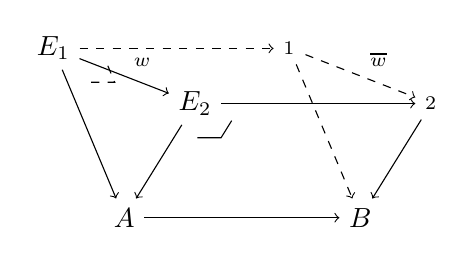
\begin{tikzpicture}[x={(1.5cm,0cm)},y={(0cm,1.8cm)},z={(1.8cm,-0.7cm)}]
  % part over A:
  \node (A) at (0,0,0) {$A$};
  \node (E1) at (0,1,-0.5) {$E_1$};
  \node (E2) at (0,1,0.5) {$E_2$};
  \draw[->] (E1) to (A);
  \draw[->] (E2) to (A);
  \draw[->,auto] (E1) to node {$\scriptstyle w$} (E2);
  % part over B:
  \node (B) at (2,0,0) {$B$};
  \node (Eb1) at (2,1,-0.5) {$\Ebar_1$};
  \node (Eb2) at (2,1,0.5) {$\Ebar_2$};
  \draw[->,dashed] (Eb1) to (B);
  \draw[->] (Eb2) to (B);
  \draw[->,dashed,auto] (Eb1) to node {$\scriptstyle \overline{w}$} (Eb2);
  % connecting arrows:
  \draw[->] (A) to (B);
  \draw[->] (E2) to (Eb2);
  \draw (0.2,0.7,0.35) -- (0.4,0.7,0.35) -- (0.4,0.85,0.425); % pullback sign
  \draw[->,dashed] (E1) to (Eb1);
  \draw[dashed] (0.2,0.8,-0.4) -- (0.4,0.8,-0.4) -- (0.4,0.9,-0.45); % pullback sign
\end{tikzpicture}\]

As usual, it is sufficient to construct this first without well-orderings on $\Ebar_1$; these can then always be chosen so as to extend those of $E_1$. \\

Recalling Lemmas~\ref{lemma:exp_along_cofib}--\ref{lemma:joyal-lemma}, we define $\Ebar_1$ and $\overline{w}$ as the pullback
 \[\xymatrix{
  \Ebar_1 \ar[d]_{\overline{w}} \ar[r] \pb & \toposPi_i E_1 \ar[d]^{\toposPi_i w} \\
  \Ebar_2 \ar[r]_{\eta}                    & \toposPi_i E_2
 }\]
in $\sSets/B$, where $\eta$ is the unit of $i^* \adjoint \toposPi_i$ at $\Ebar_2$.  To see that this construction works, it remains to show:
\begin{enumerate}[(a)]
\item $i^*\Ebar_1 \iso E_1$ in $\sSets/A$, and under this, $i^* \overline{w}$ corrsponds to $w$;
\item $\Ebar_1$ is $\alpha$-small over $B$;
\item $\Ebar_1$ is a fibration over $B$, and $\overline{w}$ is a weak equivalence.
\end{enumerate}

For (a), pull the defining diagram of $\Ebar_1$ back to $\sSets/A$; by Lemma~\ref{lemma:exp_along_cofib} part 2, we get a pullback square
\[\xymatrix{
  i^*\Ebar_1 \ar[d]_{i^*\overline{w}} \ar[r] \pb & E_1 \ar[d]^w \\
  E_2 \ar[r]^{1_{E_2}}                               & E_2
}\]
in $\sSets/A$, giving the desired isomorphism.

For (b), Lemma~\ref{lemma:exp_along_cofib} part 3 gives that $\toposPi_i E_1$ is $\alpha$-small over $B$, so $\Ebar_1$ is a subobject of a pullback of $\alpha$-small maps.

For (c), note first that by factoring $w$, we may reduce to the cases where it is either a trivial fibration or a trivial cofibration.

In the former case, by Lemma~\ref{lemma:exp_along_cofib} part 1 $\toposPi_i w$ is also a trivial fibration, and hence so is $\overline{w}$; so $\Ebar_1$ is fibrant over $\Ebar_2$, hence over $B$.

In the latter case, $E_1$ is then a deformation retract of $E_2$ over $A$; we will show that $\Ebar_1$ is also a deformation retract of $\Ebar_2$ over $B$.  Let $H \colon E_2 \times \Delta[1] \to E_2$ be a deformation retraction of $E_2$ onto $E_1$.  We want some homotopy $\Hbar \colon \Ebar_2 \times \Delta[1] \to \Ebar_2$ extending $H$ on $E_2 \times \Delta[1]$, $1_{\Ebar_1} \times \Delta[1]$ on $\Ebar_1 \times \Delta[1]$, and $1_{\Ebar_2}$ on $\Ebar_2 \times \{0\}$.  Since these three maps agree on the intersections of their domains, this is exactly an instance of the homotopy lifting extension property, i.e.\ a square-filler
\[\xymatrix{
  (E_2 \times \Delta[1]) \cup (\Ebar_1 \times \Delta[1]) \cup (\Ebar_2 \times \{0\})
     \ar@{^{(}->}[d] \ar[rr]^<>(0.4){H \cup 1 \cup 1}   % extra close-bracket to unconfuse emacs parser: )
     & & \Ebar_2 \ar[d] \\
  \Ebar_2 \times \Delta[1] \ar[rr] \ar@{.>}[urr]|{\Hbar} & & B
} \qquad \quad \]
which exists since the left-hand map is a trivial cofibration.

For $\Hbar$ to be a deformation retraction, we need to see that $\Hbar_{\{1\}} \colon \Ebar_2 \to \Ebar_2$ factors through $\Ebar_1$.  By the definition of $\Ebar_1$, a map $f \colon X \to \Ebar_2$ over $b \colon X \to B$ factors through $\Ebar_1$ just if the pullback $i^*f \colon i^*X \to E_2$ factors through $E_1$.  In the case of  $\Hbar_{\{1\}}$, the pullback is by construction $i^*(\Hbar_{\{1\}}) = (i^*\Hbar)_{\{1\}} = H_{\{1\}} \colon E_2 \to E_2$, which factors through $E_1$ since $H$ was a deformation retraction onto $E_1$.

So $\overline{w}$ embeds $\Ebar_1$ as a deformation retract of $\Ebar_2$ over $B$; thus $\Ebar_1$ is a fibration over $B$ and $\overline{w}$ a weak equivalence, as desired.
\end{proof}

Putting this together with Corollary~\ref{cor:simplicial-model}, we obtain our main theorem:
 
\begin{theorem} \label{thm:simplicial-model-univalent}
Let $\beta < \alpha$ be inaccessible cardinals.  Then there is a model of dependent type theory in $\sSets_{\UU}$ with all the logical constructors of Section~\ref{subsec:logical-rules}, and a universe (given by $\UU[\beta]$) closed under these constructors and satisfying the Univalence Axiom. \qed
\end{theorem}

From this, we can immediately deduce:

\begin{theorem} \label{thm:uf-consistent}
  Assuming the existence of two inaccessible cardinals, the contextual category presentation of $\mathsf{MLTT}+\mathsf{UA}$ (as given in Definition~\ref{def:uf-and-models}) is consistent. \qed
\end{theorem}

In practice one often considers a type theory with a sequence of $n$ or $\omega$ univalent universes. We expect that the techniques used in the proof of Theorem \ref{thm:uf-consistent} can be adapted to yield a consistency proof for such a theory, relative to set theory with suitable many inaccessible cardinals; but we do not pursue that here.

\begin{remark}
One can prove, within the type theory, that the Univalence Axiom together with the $\synPi$-$\eta$ rule implies functional extensionality; see \cite{voevodsky:univalent-foundations-coq}, \cite[Sec.~4.9]{hott:book}.  So we could have omitted functional extensionality from Proposition~\ref{prop:eta-and-funext}, and instead deduced it here as a corollary of univalence.
\end{remark} 

\subsection{Univalence and pullback representations} \label{subsec:pullback-reps}

We are now ready to give a uniqueness statement for the representation of an $\alpha$-small fibration as a pullback of ${p_\alpha} \colon \UUt \to \UU$: we define the space of such representations, and show that it is contractible. 

In fact, we work a bit more generally.  Given fibrations $q$, $p$, we define a space $\PP_{q,p}$ of representations of $q$ as a pullback of $p$; and we show that a fibration $p$ over a Kan base is univalent exactly when for every $q$, $\PP_{q,p}$ is either empty or contractible.

Let $p \colon E \to B$ and $q \colon Y \to X$ be fibrations.  We define a functor
\[ \P_{q,p} \colon \sSets^{\op} \to \Sets, \]
setting $\P_{q,p} (S)$ to be the set of pairs of a map $f \colon S \times X \to B$, and a weak equivalence $w \colon S \times Y \to f^*E$ over $S \times X$; equivalently, the set of squares
\[\xymatrix{
 S \times Y \ar[r]^{f'} \ar[d]_{S \times q} & E \ar[d]^{p} \\
 S \times X \ar[r]_{f}                     & B
}\]
such that the induced map $S \times Y \to f^*E$ is a weak equivalence.  Lemma~\ref{lemma:weqs_pull_back} ensures that this is functorial in $S$, by pullback.

\begin{lemma}
The functor $\P_{q,p}$ is representable, represented by the object 
\[ \PP_{q,p} := \toposPi_{X \shortto 1} \toposSigma_{\pi_1} \intEq_{X \times B} (\pi_1^* Y, \pi_2^* E).\]
\[ 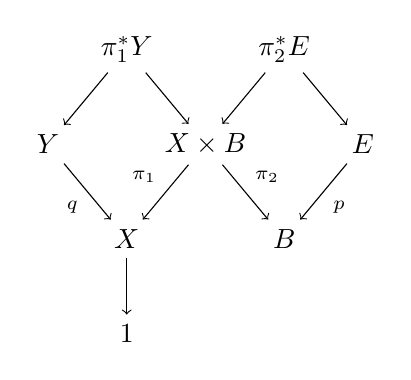
\begin{tikzpicture}[x=2cm,y=1.2cm]
\node (1) at (0,0) {$1$};
\node (X) at (0,1) {$X$};
\node (B) at (1,1) {$B$};
\node (Y) at (-0.5,2) {$Y$};
\node (E) at (1.5,2) {$E$};
\node (XxB) at (0.5,2) {$X \times B$};
\node (Y') at (0,3) {$\pi_1^* Y$};
\node (E') at (1,3) {$\pi_2^* E$};
\draw[->] (X) to (1);
\draw[->,auto,swap] (Y) to node {$\scriptstyle q$} (X);
\draw[->,auto,swap] (XxB) to node {$\scriptstyle \pi_1$} (X);
\draw[->,auto] (XxB) to node {$\scriptstyle \pi_2$} (B);
\draw[->,auto] (E) to node {$\scriptstyle p$} (B);
\draw[->] (Y') to (Y);
\draw[->] (Y') to (XxB);
\draw[->] (E') to (XxB);
\draw[->] (E') to (E);
\end{tikzpicture} \]
\end{lemma}

\begin{proof}
For any $S$, we have:
\begin{equation*}
\begin{split}
  \Hom &(S,\toposPi_{X \shortto 1} \toposSigma_{\pi_1} \intEq_{X \times B} (\pi_1^* Y, \pi_2^* E)) \\
    & \iso \Hom_X (X \times S, \toposSigma_{\pi_1} \intEq_{X \times B} (\pi_1^* Y, \pi_2^* E)) \\
    & \iso \{ (\hat{f},\hat{w})\ |\ \hat{f} \colon X \times S \to X \times B\ \text{over}\ X, \\
    & \qquad \qquad \quad \  \hat{w} \colon X \times S \to \intEq_{X \times B} (\pi_1^* Y, \pi_2^* E)\ \text{over}\ X \times B \} \\
    & \iso \{ (f,w)\ |\ f \colon X \times S \to B,\ w \colon Y \times S \to f^* E\ \text{w.e.\ over}\ X \times S \} \\
    & \iso \P_{q,p}(S) \qedhere
\end{split}
\end{equation*}
\end{proof}

\begin{remark}
By Yoneda, we see from this that $(\PP_{q,p})_n \iso \P_{q,p}(\Delta[n])$.
\end{remark}

\begin{theorem} \label{thm:univalent-characterization}
Let $p \colon E \to B$ be a fibration, with $B$ Kan.  Then $p$ is univalent if and only if for every fibration $q \colon Y \to X$, $\PP_{q,p}$ is either empty or contractible.\footnote{Constructively-minded readers might prefer to phrase this as: if $\PP_{q,p}$ is inhabited, then it is contractible.  In the language of \cite{hott:book}, it is a \emph{mere proposition}.}
\end{theorem}

\begin{proof}
First, suppose that $p$ is univalent.  Take any $q$ such that $\PP_{q,p}$ is non-empty; then we have some map $1 \to \PP_{q,p}$, corresponding to a square
\[ 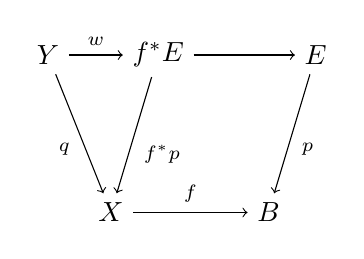
\begin{tikzpicture}[x=2cm,y=2cm]
\node (X) at (0,0) {$X$};
\node (B) at (1,0) {$B$};
\node (Y) at (-0.4,1) {$Y$};
\node (f*E) at (0.3,1) {$f^*E$};
\node (E) at (1.3,1) {$E$};
\draw[->,auto] (X) to node {$\scriptstyle f$} (B);
\draw[->,auto,swap] (Y) to node {$\scriptstyle q$} (X);
\draw[->,auto] (f*E) to node {$\scriptstyle f^*p$} (X);
\draw[->,auto] (E) to node {$\scriptstyle p$} (B);
\draw[->,auto] (Y) to node {$\scriptstyle w$} (f*E);
\draw[->] (f*E) to (E);
\end{tikzpicture} \]

We claim that $\PP_{q,p} \to 1$ is a trivial fibration, and hence $\PP_{q,p}$ is contractible.  $\toposPi$-functors preserve trivial fibrations (since their left adjoints, pullback, preserve cofibrations), so it is enough to show that 
\[\intEq_{X \times B} (\pi_1^* Y, \pi_2^* E) \to X \times B \to^{\pi_1} X\]
is a trivial fibration.

For this, first note that $w$, as a weak equivalence between fibrations, is a homotopy equivalence over $X$, so induces a homotopy equivalence 
\[(w\cdot -) \colon \intEq_{X \times B} ((\pi_1^* (f^* E), \pi_2^* E) \to \intEq_{X \times B} (\pi_1^* Y, \pi_2^* E).\]
 So it is enough to show that $\intEq_{X \times B} ((\pi_1^* (f^* E), \pi_2^* E) \to X \times B \to^{\pi_1} X$ is a trivial fibration; but this follows since it is the pullback along $f$ of the “source” map $\intEq(E) = \intEq_{B \times B}(\pi_1^*E,\pi_2^*E) \to B \times B \to^{\pi_1} B$, which is a trivial fibration since $p$ is univalent and $B$ is Kan.

Conversely, suppose that for every fibration $q$, $\PP_{q,p}$ is either empty or contractible; now, we wish to show $p$ univalent.  For this, it is enough to show that the source map $s \colon \intEq(E) \to B$ is a trivial fibration, which will hold if each of its fibers is contractible.

So, take some $f \colon 1 \to B$, and consider the fiber $f^*\intEq(E)$.  By the universal property of $\intEq(E)$, this is isomorphic to $\PP_{f^*p,p}$; and it is certainly non-empty, containing the pair $(f, 1_{f^*E})$; so by assumption, it is contractible, as desired.
\[ \begin{gathered}[b]
  \xymatrix{
    f^* \intEq(E) \ar[r] \ar[d] \pb & \intEq(E) \ar[d]^s \\
    1 \ar[r]^f & B
  } \\[-\dp\strutbox]
\end{gathered} \qedhere
\]
\end{proof}

\begin{corollary}
For any $\alpha$-small fibration $q$, the simplicial set $\PP_{q, p_\alpha}$ of representations of $q$ as a pullback of $p_\alpha$ is contractible. \qed
\end{corollary}



%%% Local Variables:
%%% mode: latex
%%% TeX-master: "simplicial-model"
%%% End: 